Веб-приложение, использующее аппаратную графику, имеет несколько иную структуру, нежели классическое веб-приложение ввиду его разделение на две уединенные части -- часть,
отвечающую за отображение пользовательского интерфейса в HTML (часть, пресущую всем веб-приложениям), и часть отображения трехмерной графики (рисунок \ref{figure:theory:webgl_app}).
Разрабатываемая система подразделяется на компоненты исходя из их целевого назначения и разные компоненты имеют строго уединенные зависимости.

\begin{figure}[ht]
\centering
  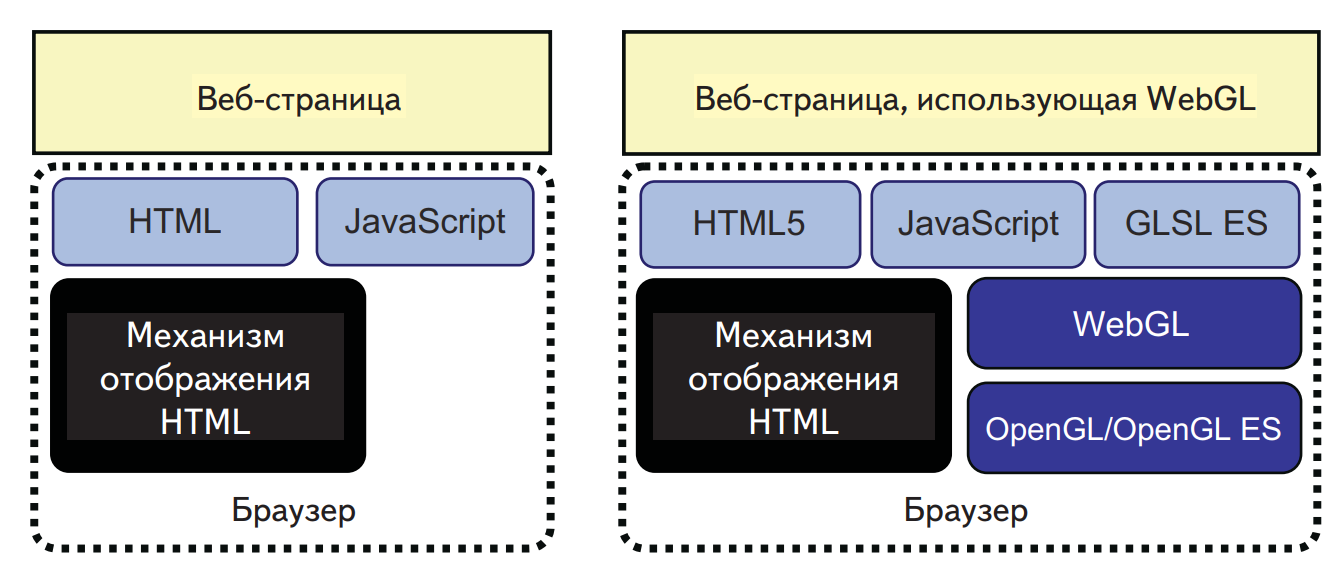
\includegraphics[scale=0.35]{web_with_webgl.png}
  \caption{Отличие приложения для отображения трехмерой графики от классического веб-приложения.}
  \label{figure:theory:webgl_app}
\end{figure}

Типичная модель приложения, производящего CRUD-операции (Create, Read, Update, Delete) обычно содержит в себе набор связанных между собой модулей,
имеющих строго определенные на этапе компиляции связи. Поскольку разрабатываемая система является частным случаем CRUD-системы (без возможности удаления
пользовательского содержимого), то схожая декомпозиция системы может быть применена и для нее. Разрабатываемая система условно подразделяется на следущие модули:

\subsubsection{Компонент отображения}
\label{sub:theory:components:rendering}

Основное назначение компонента отображения -- собственно вызов низкоуровневых API WebGL, итерация по вершинам трехмерной модели и их добавление в контекст
отображения WebGL. Также данный компонент служит для контроля над материалами и шейдерами для отображения различных элементов трехмерной модели.
Данный компонент имеет зависимость от стороннего модуля threejs, который упаковывается вместе с остальными сторонними библиотеками и подключается к
приложению динамически.

Основные части компонента отображения:

\begin{itemize}
\item CanvasRenderer -- модуль, занимающийся непосредственной манипуляцией вершинами трехмерной модели при ее отображении.
\item MaterialPicker -- модуль-описатель свойств материалов, содержит в себе описания всех шейдеров, необходимых для отображения материалов.
\item GeometryIterator -- модуль, предназначенный для итерации по вершинам трехмерной модели для последующего отображения его в CanvasRenderer.
\end{itemize}

Публичный интерфейс компонента состоит из следующих методов:
\begin{itemize}
\item setRenderingModel(modelInfo) -- устанавливает модель для отображения из информации о модели. Аргумент modelInfo -- объект-описатель геометрии отображаемого объекта;
\item render(cameraInfo) -- непосредственно отображает модель на canvas. Аргумент cameraInfo -- трансформ-сущность камеры (ее положение в пространстве и поворот), тип камеры (орто, перспектива);
\item clearScreen() -- очищает экран.
\end{itemize}

\subsubsection{Компонент геометрических вычислений}
\label{sub:theory:components:calculation}

Основное назначение компонента геометрических вычислений -- произведение функциональных манипуляций над точками в трехмерном пространстве, преобразования вершин трехмерной модели, применение
фундаментальных трансформаций к точкам (трансляция, поворот, масштабирование) и реализация вспомогательных математических операций для работы с трехмерной сценой. Данный компонент имеет стороннюю
зависимость от стандартной библиотеки математики JavaScript.Math и от модуля underscore (lodash) для функциональной работы с коллекциями данных и векторами.

Основные части компонента графических вычислений:

\begin{itemize}
\item VectorTranslator -- модуль, реализующий операцию трансляции векторов. Использует библиотеки векторной манипуляции underscore, lodash;
\item VectorRotator -- модуль, реализующий операцию поворота вектора на определенный угол относительно определенной оси. Реализует операции поворота с помощью кватернионов;
\item VectorScaler -- модуль, реализующий операцию масштабирования вектора относительно начала координат или другой произвольной точки;
\item QuaternionHelper -- вспомогательный модуль реализующий арифметические операции над кватернионами и трехмерными векторами. Используется в VectorRotator и является частью публичного интерфейса
данного компонента;
\item VectorHelper -- вспомогательный модуль, реализующий арифметические операции над трехмерными векторами. Используется во всех подсистемах компонента графических вычислений и также является частью 
публичного интерфейса данного компонента;
\item VectorProjector -- модуль-аггрегатор поведения других модулей, реализующих стандартные операции. Реализует преобразования проекций трехмерной модели до отображения ее на экране.
\end{itemize}

Публичный интерфейс компонента состоит из следующих методов и вспомогательных типов:
\begin{itemize}
\item класс VectorHelper -- реализующий армифметику над векторами;
\item класс QuaternionHelper -- реализующий армифметику над кватернионами и векторами;
\item performMVProjection(model, camera) -- реализует проецирование трехмерной модели из пространства сцены в пространство камеры.
\end{itemize}

\subsubsection{Компонент пользовательского интерфейса}
\label{sub:theory:components:ui}

Основное назначение компонента пользовательского интерфейса (Компонента UI) -- реализация возможностей по манипулации состоянием приложения для пользователя, оргазинация
контрольных элементов для вызова функций приложения.
Компонент UI отвечает за управление пользовательским интерфейсом системы и содержит ряд интерфейсов-контрактов и классов для взаимодействия с прочими компонентами
с большой степенью абстракции. Компонент UI предоставляет внешним модулям интерфейс \texttt{IUIDisplayable}, объявляющий метод обязанный реализовать набор правил
по установлению связи между доменной абстракцией системы и объектом, являющимся его моделью отображения.

Компонент UI будучи точной входа в React-приложение (и в приложение в целом), имеет большое число вспомогательных модулей, поэтому перечисление их всех не представляется целесообразным.
Следует также обратить внимание на тот факт, что в терминах Reactjs, модули пользовательского интерфейса также именуются компонентами, что вносит некоторую двусмысленность в перечисление списка
подмодулей компонента UI. Далее в этом списке под компонентом имеются в виду React-компоненты. Фактически, в рамках компонента реализуется модуль на каждый элемент пользовательского 
интерфейса, такой как кнопка или элемент меню. Ниже представлены основные элементы данного компонента:

\begin{itemize}
\item AppComponent -- фактическая точка входа в приложение, является объектом вызова ReactDOM.render и контейнером всех остальных систем.
\item BasicOperationsComponent -- дочерний к AppComponent элемент, является контейнером элементов пользовательского интерфейса, отвечающих за вызов базовых преобразований трехмерной
модели -- трансляции, поворота и масштабирования.
\item MainMenuComponent -- дочерний к AppComponent элемент, реализующий стандартное меню приложения и доступ к глобальным базовым функциям приложения (например, загрузка и выгрузка моделей).
\end{itemize}